\documentclass[11pt, oneside]{article}   	% use "amsart" instead of "article" for AMSLaTeX format
\usepackage{geometry}                		% See geometry.pdf to learn the layout options. There are lots.
\geometry{a4paper}                   		% ... or a4paper or a5paper or ... 
%\geometry{landscape}                		% Activate for rotated page geometry
%\usepackage[parfill]{parskip}    		% Activate to begin paragraphs with an empty line rather than an indent
\usepackage{graphicx}				% Use pdf, png, jpg, or eps§ with pdflatex; use eps in DVI mode
								% TeX will automatically convert eps --> pdf in pdflatex		
\usepackage{amssymb}
\usepackage{amsmath}
\usepackage{authblk}
\usepackage[hyphens]{url}

\usepackage{url}
\usepackage{hyperref} 

\usepackage{titlesec}

\usepackage{caption}


\title{Ecosystem Management: From Alarm to Action}
\author{Aidan T. Parkinson; Andreea M. Benu}

\date{\today}							% Activate to display a given date or no date

\begin{document}
\maketitle
\begin{center}
\href{mailto:aidan.parkinson@gmail.com}{aidan.parkinson@gmail.com}
\end{center}

\section{Unsustainability}

At times it seems that there is nothing more captivating than territorial disputes within broadcast media.
Whether in relation to the Realpolitik of armed conflicts, penalty attributions for climate change or attempting to define what sustainable development means for themselves.
Such disputes rarely appear a domain for inspirational reason and struggle to be much of an example to follow.
Within such a context, one may seek common society founded upon ideal principles through individual agreements.
A good example of such efforts is the work of John Rawls in \emph{"The Law of Peoples"}.
However, whilst such contracts may appear ideal, they appear incomplete.\\

Rawls acknowledges that \emph{"Peoples have a duty to assist other Peoples living under unfavourable conditions that prevent their having a just or decent political and social regime."}
However, he seems to neglect the reality that everyone apparently lives under unfavourable conditions and, hence, has an obligation of service to the commons.
Is it realistic that such an ideal society wouldn't be subject to an imperfect system of Nation States?
Could a State of Nature be the root cause of such an imperfect regime?
How could such a State of Nature be defined?
If one were subject to such a regime, could there be a social expectation to serve in the common interest?
What reasonable actions could an individual take to effectively serve?
How could such actions be implemented, so as to develop a reasonable community?\\

There appears substantial duty that can be realised by simply paying attention to ones homework.
A duty apparently shared by all, whatever ones walk of life.
The outcome of such a perspective is a \emph{"best we can do society"}, rather than anything approaching Rawls's \emph{"ideal society of Peoples"}.
Our argument is that the \emph{"best we can do society"} actually provides the more complete form of contract that Rawls followers would need to meet their ends.
What follows is a paper intended to set out a new and reasonable theoretical framework, underpinned by the idea of a \emph{"Commonwealth of Peoples"}.
Such a framework is designed so that followers can take effective action in the interest of one global commons, with minimal attendance to the Realpolitik of Nation States.
It is focussed on demand-side assurance and investment advisory to private entities, whilst holding a global perspective.
Providing a platform that has the potential to universally scale across all end-use services.\\

One begins this investigation by establishing an understanding of common ecosystem performance, identifying methods for making an \emph{"Ecosystem Performance Observation"}.
This is followed by developing a suitable cost-benefit ratio for \emph{"Service Ratings}, with careful application of the Ecosystem Performance Observation formulae.
Further, Service Ratings may be benchmarked against peers and compared to inform tailored service investment advice.
This theoretical framework is supported with worked examples for each indicator, together with some ideas of suitable technologies for application.\\

\section{Ecosystem Performance Observations}

When examining carbon-based life, such as humans, it is natural to take an interest in their activities and bi-products.
Certain items of waste, such as consumer goods packaging and water quality, might be tended well by the authorities of territories.
However, when all accounted for greenhouse gas emissions are a by-product of any human agreement anywhere.
Such anthropogenic emissions are vented to a common ecosystem, for which many might expect an equitable share.
The state of our common ecosystem on planet Earth is maintained by carbon sinks that absorb the greenhouse gas emissions of anthropogenic activities.
A common misunderstanding here is to exclude energy management activities in ecosystem development from our understanding of carbon sinks.
One can easily consider human intellect as a plausible carbon sink.
In fact all \emph{"Enablement Assets"} have both the potential to manage down greenhouse gas emissions and be distributed as software.
There is no way to delegate responsibility for energy management.
Energy management effects every decision and agreement one makes, to include the most senior occupations.
A goal of economic growth has more relevance to the successful servicing of national debts.
But, it is the state of our carbon sinks that could be a more interesting measure of overall ecosystem performance.\\

Under consideration are common agreements between individuals, not Nation States or territories.
Such agreements require a constitution, without legal dependencies.
John Rawls \emph{"The Law of Peoples"} is a credible candidate.
However, we have determined an additional minimum service in common that relates to ecosystem performance.
Such service performance observations are necessary, as humans have considerable capacity to cause damage through Realpolitik or error.
So, how could such observations be made?

\subsection{Utilitarian Perspective}

Calculation of a Social Cost of Carbon to measure the state of the ecosystems carbon sinks has proven to be highly rewarding for those taking utilitarian perspectives, prescribing happiness as a whole as the ultimate end to action ~\cite{hs1}.
The resources consumed in satisfying human needs require economic considerations to efficiently manage personal well-being. Normative economists often regard only individual circumstance, or level of  welfare, in a state of affairs as important.
This is known as the neutrality assumption~\cite{pd2}.
Arrow, May and Sen assert that this position of neutrality is effectively an avocation of anonymity with respect to social states, which is a requirement that human beings be treated equally~\cite{ka1}~\cite{km1}~\cite{as2}.
Waldron defines the notion of social welfare, an aggregate of individual welfare, as being goal-based~\cite{jw2}.
Dworkin states that a goal can be considered a non-individuated political aim~\cite{rd1}.\\

Early contributions to address this research question were awarded the Nobel Prize~\cite{np1} and Life peerages in the House of Lords~\cite{g1}.
These notable precedents prescribe aggregate or social welfare as a goal for social benefit.
Aggregate welfare is not evenly distributed amongst the worlds population.
In 2019, Business Insider magazine reported that the 26 richest men had more combined wealth than the poorest 3.8 billion people on Earth~\cite{bi1}.
Therefore, pure reinforcement of aggregate welfare is largely in the interest of a few wealthy people.
This approach typically employs Frank Ramsey's Mathematical Theory of Saving as a decision-making tool.
The process involves creating complex integrated assessment models of humanities social and environmental systems that apply gross assumptions of Earth's development.
Mechanisms that determine the state of the world are identified and the consequences of alternative policies charted so that consequences can be valued.
Welfare surpluses are then estimated for policy options, by making projections of differences from the \emph{status quo} 100's of years into the future.
Valuation of these surpluses involves setting a global social discount rate and this requires a set of personal assumptions~\cite{pd2}.
A summary of the underlying decision-making criteria is shown follows~\cite{fr1}:\\

\begin{equation}
V_t = \sum_t^\infty \beta^{(\tau - t)} \cdot U (C_\tau)
\qquad \text{for }
\qquad t \geq 0
\end{equation}

Where,
\begin{equation}
\beta = \frac{1}{(1+\mu)}
\end{equation}

Where, $V_t$ is \emph{a generations welfare}, $\beta$ is the \emph{discount factor}, $U$ is \emph{welfare}, $C_\tau$ is \emph{consumption during time-step}, $t$ is \emph{time} and $\mu$ the \emph{social discount-rate}.\\

\begin{equation}
\mu = \sigma \cdot g + \delta
\end{equation}

Where, $\sigma$ is the \emph{marginal utility of consumption} and the difference in the utility one would gain from a unit of consumption by those of low and high incomes, $g$ is the \emph{long-term growth rate} in consumption, $\delta$ is the \emph{pure rate of time preference} and our impatience to consume in fear of extinction.\\

\begin{equation}
S = \frac{\mu-\delta}{\sigma \cdot \mu}
\end{equation}

Where, $S$ is the \emph{savings rate} and the proportion of output that should be invested.\\

In practical applications, $U (C_\tau)$ can be substituted for net cash-flow in time period to yield a familiar equation.\\

This complex process results in considerable disagreement amongst Social Cost of Carbon estimates for a historic time period using this method.
The assumptions for a global social discount rate used for three notable contributions are provided in Table~\ref{Social contributions table}.
The global social discount rate for these three contributions ($\mu$) is similar.
However Cline is outlying in estimation of the difference in utility the wealthy gain from a unit of consumption compared to the poor ($\sigma$).
None of the three contributions agree on a long-term global growth rate ($g$).
When considering impatience to consume in fear of extinction ($\delta$) it is Nordhaus that appears outlying.
This yields very different values for the amount of surplus to be saved relative to that consumed amongst the three contributions ($S$).
Clearly the worlds envisioned by just these three notable precedents are really quite different in nature and perhaps the reality is that the ethical positions of these contributors are in competition.
Nobody has the power in reality to set a social discount rate in this way for all society.
For most, the setting of these assumptions is of private preference only.\\

\begin{table}[H]
\caption{Notable Precedents: Assumptions in Social Discounting}
\begin{center}
\begin{tabular}{| l | c | c | c | c | c |}
\hline
Contribution&$\mu$&$\sigma$&$g$&$\delta$&$S$\\
\hline
Cline, 1992~\cite{wc1}&0.05&1.5&0.033&0&0.67 \\
Nordhaus, 1994~\cite{wn1}&0.05&1&0.02&0.03&0.4 \\
Stern, 2006~\cite{ns1}&0.05&1&0.049&0.001&0.98 \\
\hline
\end{tabular}
\end{center}
\label{Social contributions table}
\end{table}

Figure~\ref{USA SCC figure} is a graphical representation of Social Cost of Carbon estimates by the Interagency Working Group on Social Cost of Carbon, United States Government.
This meta-analysis considers the results of three pioneer integrated assessment models developed in the 1990's.
These are the DICE, PAGE and FUND models~\cite{wn1}~\cite{ch1}~\cite{rsjt1}.
The modelling simulations considered by this study returned a Social Cost of Carbon anywhere between $<$2007\$0tC\textsuperscript{-1} to a 95th percentile of 2007\$128tC\textsuperscript{-1} with $\mu$ set at 0.03~\cite{iwg1}.
Based upon these results for a Social Cost of Carbon, it is clear that utilitarians would find it difficult to significantly alter their actions and agree on options to be taken. \\

\begin{figure}[H]
\centering
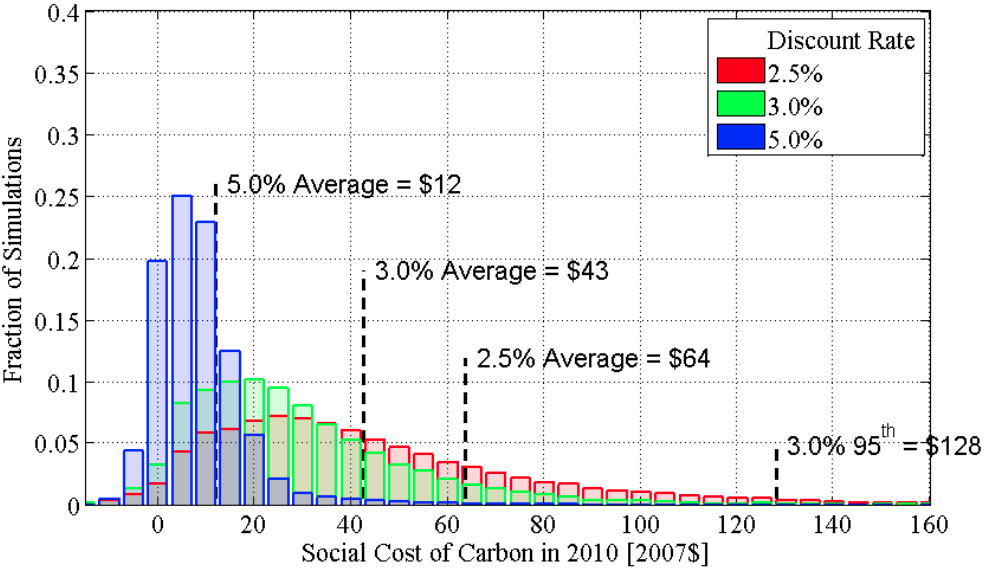
\includegraphics[width=1\textwidth]{scc}
\caption{Social Cost of Carbon in 2010 (in 2007 dollars per metric ton)}
\label{USA SCC figure}
\end{figure}

\begin{quote}
"Here there are a number of possibilities. A collective decision may determine the rate of saving while the direction of investment is left largely to individual firms competing for funds. In both a Private Property as well as in a socialist society great concern may be expressed for preventing irreversible damages and for husbanding natural resources and preserving the environment. But again either one may do rather badly."~\cite{jr1}
\end{quote}

Even among welfare economists, some reject applying pure time preference so that one allows the living to take advantage of their position in time to favour their own interests~\cite{hs1}~\cite{fr1}.
Such examples ignore the possibility for the living to wrong their predecessors or descendants.
Dasgupta argues that it is one thing to urge that an imperfect economy should be improved, quite another to pretend that the imperfect economies we inhabit are Utopia in the way these contributions suggest.
Collective saving for the future has many aspects of a Public Good, though under conditions of arising problems of isolation and assurance~\cite{as1}~\cite{ms1}.
Those who follow the principles of the social contract when taking action would probably find these methods have little relevance to their sense of justice.
These contributions also do not consider the possibility for states of affairs to deliver imperfect procedural justice leading to noncompliance.
Libertarian's might argue that such collective action would lead to violations of individual rights to even a slight extent and therefore should be rejected~\cite{rn1}.
Advocates of the free-market may criticise such methodologies that involve seeking prosperity through centralised long-term coercive planning, rather than appropriate regulation that allows local agents to adjust their activities according to the present situation~\cite{fh1}.
There is indeed nothing sacrosanct about the Public decision concerning the level of savings and its bias with respect to time preference deserves no special respect~\cite{jr1}.
Therefore, an alternative proposition is sought.\\

\subsection{Hobbesian Perspective}

An alternative perspective is to use the principles of the social contract to estimate a \emph{"Commonwealth Cost of Carbon"} for decision-making.
Here, one cannot rely on the assumption that the ideals of liberal democracy or social welfare are necessarily shared by all those affected.
However, one might assume acknowledgement between parties of an ecosystem represented by a Hobbesian \emph{"State of Nature"} with allowances for error and Realpolitik.\\
The problem is to use Hobbesian thought to value the common cost of greenhouse gas emissions.
Dasgupta asserts that this valuation need involve comparison of worlds with and without greenhouse gas emissions and stable currency~\cite{pd2}.\\

Ones understanding of the carbon cycle helps us determine that a world without greenhouse gas emissions is a world without life.
The Moon is an example of a world without a significant carbon cycle.
Carbon emissions appear an essential good that life cannot do without.
What becomes important is not the quantity of greenhouse gas emissions, but the quality of greenhouse emissions.\\

The next task is to understand what a world would be like without stable currency.
Hobbes would suggest this be a war of \emph{all against all}, a world without submission to a Sovereign power.
There is currently no widely recognised Sovereign power in existence, although there have been various attempts over time.
Hence, currency isn't as stable as it could be and wars do present themselves regularly.
Nevertheless, there is no reason why such an endeavour might not be a common goal and couldn't be proposed.
To maintain confidence, citizens of a well-ordered society will normally want the rule of law maintained.
Although we might acknowledge that a common sense of justice is shared and that each wants to adhere to its arrangements, one might nevertheless lack full confidence in one another.
One might suspect that others are not doing their part, and so may be tempted not to do theirs.
The general awareness of these temptations may cause social systems to break down.
The role of an public interpretation of rules supported by collective sanctions is needed precisely to overcome this instability.
For this reason alone, a coercive state appears always necessary, even though in a well-ordered society sanctions may be slight and may never need be imposed.
Therefore, the penal machinery of state becomes ones security to another and is entirely sacrificial~\cite{jr1}.\\

Therefore, in order to optimise ones actions to assure \emph{faith in promise}, one arrives at an ecosystem performance observation equivalent to a \emph{Commonwealth Cost of Carbon} for a given time-period:\\

\begin{equation}
	\frac{anthropogenic\; expenditure\; on\; enforcement}{anthropogenic\; greenhouse\; emissions}
\end{equation}

It is evident that this calculation method requires relatively straightforward math, but the accounting is not trivial.\\


\section{Service Ratings}


\section{Conclusions}


\end{document}